%----------------------------------------------------------------------------
\section{Stylized Facts}
%----------------------------------------------------------------------------

\begin{frame}

\begin{center}
{\LARGE Stylized Facts}
\end{center}

\end{frame}

%%%%%%%%%%%%%%%%%%%%%%%%%%%%%%%%%%%%%%%%%%%%%%%%%%%%%%%%%%%%%%%%%%%%%%%%%%%%%
%%%%%%%%%%%%%%%%%%%%%%%%%%%%%%%%%%%%%%%%%%%%%%%%%%%%%%%%%%%%%%%%%%%%%%%%%%%%%

\begin{frame}{Macroeconomic fluctuations}

Decomposing fluctuations
	\begin{itemize}
	\item Underlying trend / low-frequency movements (`growth' literature)
	\item Business cycle
	\item Measurement error
	\item Seasonality (rarely discussed - let the statisticians handle it)
	\item `Random' fluctuations (`unmodelable' - or stuff we've failed to model)
	\end{itemize}
\vspace{3mm}
Growth and fluctuations can be connected as high frequency decisions can influence low frequency phenomena
	\begin{itemize}
	\item	Consume/save/innovate $\rightarrow$ investment/technology $\rightarrow$ growth
	\item	We will focus mainly on `business cycle' fluctuations
	\end{itemize}

\end{frame}

%%%%%%%%%%%%%%%%%%%%%%%%%%%%%%%%%%%%%%%%%%%%%%%%%%%%%%%%%%%%%%%%%%%%%%%%%%%%%
%%%%%%%%%%%%%%%%%%%%%%%%%%%%%%%%%%%%%%%%%%%%%%%%%%%%%%%%%%%%%%%%%%%%%%%%%%%%%

\begin{frame}{Macroeconomic data}

\begin{figure}
\caption[GNP-PCE]{Log GNP and consumption}
\centering
\label{fig:gnp_pce}
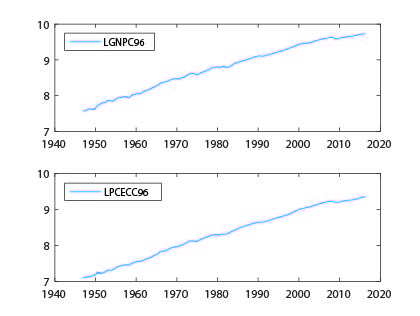
\includegraphics[width=0.45\textwidth]{Figures/gnp_pce.JPG}
\end{figure}

\begin{itemize}
\item	Note the fairly (until recently?) constant trend
\item	Long run co-movement between $Y$ and $C$
\item	Fluctuations around trend with a few big hits (recessions)
\end{itemize}

\end{frame}

%%%%%%%%%%%%%%%%%%%%%%%%%%%%%%%%%%%%%%%%%%%%%%%%%%%%%%%%%%%%%%%%%%%%%%%%%%%%%
%%%%%%%%%%%%%%%%%%%%%%%%%%%%%%%%%%%%%%%%%%%%%%%%%%%%%%%%%%%%%%%%%%%%%%%%%%%%%

\begin{frame}{Hodrick-Prescott Filter}

\href{https://en.wikipedia.org/wiki/Hodrick\%E2\%80\%93Prescott_filter}{Hodrick-Prescott filter} decomposes $y_{t}$ into trend, $\tau _{t}$, and cycle, $c_{t}$
\begin{equation*}
y_{t}=\tau _{t}+c_{t}
\end{equation*}

Trend should be `smooth' but track data closely in longer run
\begin{equation*}
\underset{\left\{ \tau _{t}\right\}_{t=1}^{T}}{\min}\left( \underbrace{\sum_{t=1}^{T}(y_{t}-\tau _{t})^{2}}_{Tracking}+\lambda \underbrace{\sum_{t=2}^{T-1}\left[ \left( \tau _{t+1}-\tau _{t}\right) -\left( \tau
_{t}-\tau _{t-1}\right) \right] ^{2}}_{Smoothness} \right)
\end{equation*}

$\lambda$ is weighting parameter
	\begin{itemize}
	\item $\lambda =0$ means $\tau _{t}=y_{t}$ and trend is data
	\item $\lambda \rightarrow \infty $ means $\Delta^{2}\tau_{t}=0$ and trend is linear
	\end{itemize}

\end{frame}

%%%%%%%%%%%%%%%%%%%%%%%%%%%%%%%%%%%%%%%%%%%%%%%%%%%%%%%%%%%%%%%%%%%%%%%%%%%%%%
%%%%%%%%%%%%%%%%%%%%%%%%%%%%%%%%%%%%%%%%%%%%%%%%%%%%%%%%%%%%%%%%%%%%%%%%%%%%%%

\begin{frame}{Hodrick-Prescott filter}

\begin{figure}
\caption[HP Trends]{Trend GNP using H-P filter}
\centering
\label{fig:gnp_different_hp}
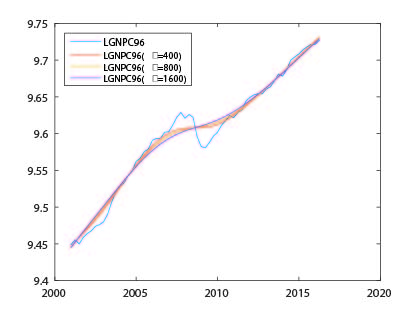
\includegraphics[width=0.35\textwidth]{Figures/gnp_different_hp.JPG}
\end{figure}

US GNP and H-P trends with different $\lambda$
\begin{itemize}
	\item	See \href{https://onlinelibrary.wiley.com/doi/abs/10.1002/jae.3950080302}{Harvey and Jaeger (1993)} on (in)appropriate use of HP filter
\end{itemize}
There are other ways of extracting trends
	\begin{itemize}
	\item	Linear (`draw a line through it')
	\item	Quadratic or cubic (`draw a bendy line through it')
	\item	Theoretical, rather than statistical (`use a model')
	\end{itemize}

\end{frame}

%%%%%%%%%%%%%%%%%%%%%%%%%%%%%%%%%%%%%%%%%%%%%%%%%%%%%%%%%%%%%%%%%%%%%%%%%%%%%%
%%%%%%%%%%%%%%%%%%%%%%%%%%%%%%%%%%%%%%%%%%%%%%%%%%%%%%%%%%%%%%%%%%%%%%%%%%%%%%

\begin{frame}{Hodrick-Prescott filter}

\begin{figure}
\caption[Power Transfer Function]{PTF of H-P filter with $\lambda =6400$ dots; $1600$ solid; $400$ dashes}
\centering
\label{fig:hp_ptf}
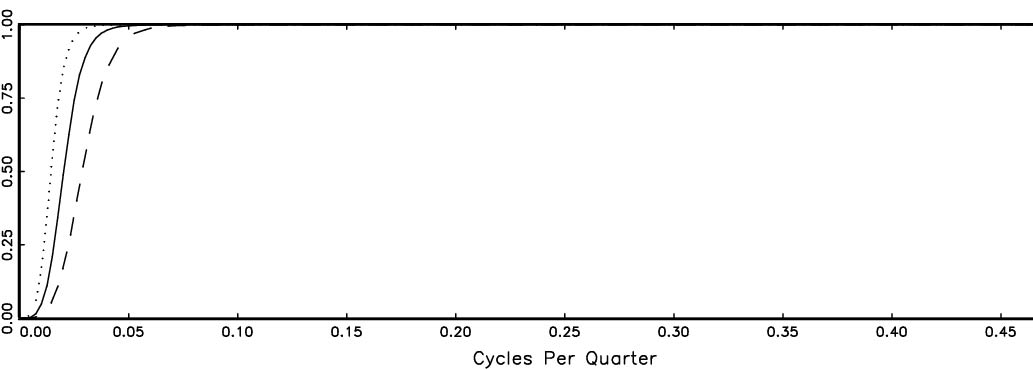
\includegraphics[width=0.40\textwidth]{Figures/hp_ptf.JPG}
\end{figure}

The \href{https://en.wikipedia.org/wiki/Filter_(signal_processing)\#The_transfer_function}{`power transfer function'} shows at what frequencies the \href{https://en.wikipedia.org/wiki/Filter_(signal_processing)}{filter} allows variation (e.g. $0.05$ cycles per quarter $\Rightarrow$ 5 years for a cycle)
	\begin{itemize}
	\item	Low frequencies: Few cycles per quarter (medium-long term trends)
	\item	High frequencies: Many cycles per quarter (business cycles and noise)
	\item	Variation in $y_{t}$ is a mix of \textit{all} frequencies - the filter lets through (\href{https://en.wikipedia.org/wiki/High-pass_filter\#/media/File:75_Hz_HPF_on_Smaart.jpg}{`passes'}) only a subset
	\end{itemize}
(Somewhat unconvincing) consensus that $\lambda =1600$ distinguishes `business cycle' and trend (quarterly data)
	\begin{itemize}
	\item	See also \href{https://www.mitpressjournals.org/doi/10.1162/003465399558454}{Baxter and King (2006)} \href{https://en.wikipedia.org/wiki/Band-pass_filter}{`band-pass'} filter
	\end{itemize}

\end{frame}

%%%%%%%%%%%%%%%%%%%%%%%%%%%%%%%%%%%%%%%%%%%%%%%%%%%%%%%%%%%%%%%%%%%%%%%%%%%%%%
%%%%%%%%%%%%%%%%%%%%%%%%%%%%%%%%%%%%%%%%%%%%%%%%%%%%%%%%%%%%%%%%%%%%%%%%%%%%%%

\begin{frame}{Long run properties of macro data}

\begin{figure}
\caption[HP Trend Growth Rate]{GNP and Trend Growth Rate ($\lambda=1600$)}
\centering
\label{fig:gnp_hp_trend}
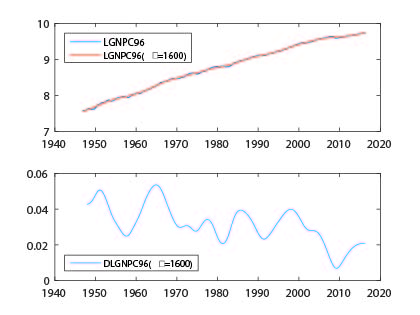
\includegraphics[width=0.40\textwidth]{Figures/gnp_hp_trend.JPG}
\end{figure}

Trend US growth `traditionally' thought of as $\approx 2.5-3.0\%$
	\begin{itemize}
	\item	GNP follows `straight line' in logs
	\end{itemize}
Note: Current debate about secular stagnation etc.
	\begin{itemize}
	\item	In U.S. labor force growth slowing and effects of `internet' subsiding
	\item	See \href{https://www.frbsf.org/economic-research/publications/economic-letter/2019/june/is-slow-still-new-normal-for-GDP-growth/}{Fernald and Li (2019)}
	\end{itemize}

\end{frame}

%%%%%%%%%%%%%%%%%%%%%%%%%%%%%%%%%%%%%%%%%%%%%%%%%%%%%%%%%%%%%%%%%%%%%%%%%%%%%%
%%%%%%%%%%%%%%%%%%%%%%%%%%%%%%%%%%%%%%%%%%%%%%%%%%%%%%%%%%%%%%%%%%%%%%%%%%%%%%

\begin{frame}{Long run properties of macro data}

\begin{figure}
\caption[Labor share and Great ratios]{Labor share and `Great Ratios'}
\centering
\label{fig:shares_ratios}
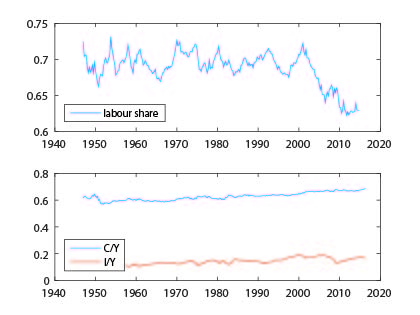
\includegraphics[width=0.30\textwidth]{Figures/shares_ratios.JPG}
\end{figure}

Fraction of output that goes to labor approximately constant
	\begin{itemize}
	\item	Or is it? \href{https://blogs.imf.org/2017/04/12/drivers-of-declining-labor-share-of-income/}{Big debate currently about declining ratio.}
	\item	Change in bargaining power, skills biased technical change, declining competition, \href{https://www.nber.org/papers/w19136.pdf}{cheaper investment goods}, \href{https://www.brookings.edu/bpea-articles/the-decline-of-the-u-s-labor-share/}{off-shoring}?
	\end{itemize}
`Great Ratios' (consumption and investment shares) $\approx$ constant
	\begin{itemize}
	\item	Maybe minor trend but these seem to be holding steady
	\end{itemize}

\end{frame}

%%%%%%%%%%%%%%%%%%%%%%%%%%%%%%%%%%%%%%%%%%%%%%%%%%%%%%%%%%%%%%%%%%%%%%%%%%%%%%
%%%%%%%%%%%%%%%%%%%%%%%%%%%%%%%%%%%%%%%%%%%%%%%%%%%%%%%%%%%%%%%%%%%%%%%%%%%%%%

\begin{frame}{Kaldor (1957) facts}

Kaldor's (1957) stylized facts have held up fairly well (subject to above caveats):
	\begin{enumerate}
	\item Output per worker grows at a roughly constant rate
	\item Capital per worker grows over time
	\item Capital/output ratio is roughly constant
	\item Rate of return to capital is constant
	\item Shares of capital and labor in net income are nearly constant
	\item Real wage grows over time
	\item Ratios of consumption and investment to GDP are constant
	\end{enumerate}

\end{frame}

%%%%%%%%%%%%%%%%%%%%%%%%%%%%%%%%%%%%%%%%%%%%%%%%%%%%%%%%%%%%%%%%%%%%%%%%%%%%%%
%%%%%%%%%%%%%%%%%%%%%%%%%%%%%%%%%%%%%%%%%%%%%%%%%%%%%%%%%%%%%%%%%%%%%%%%%%%%%%

\begin{frame}{Short run properties of macroeconomic data}

\begin{figure}
\caption[Detrended GNP and Consumption]{HP-Detrended GNP and Non-durable Consumption}
\centering
\label{fig:gnp_pce_hp_cycle}
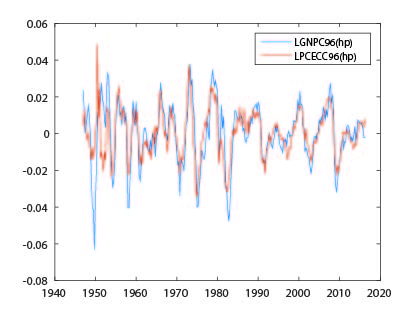
\includegraphics[width=0.55\textwidth]{Figures/gnp_pce_hp_cycle.JPG}
\end{figure}
\begin{itemize}
\item	Both series are `cyclical' components from HP filtering
\item	Strong positive correlation (consumption is `pro-cyclical')
\item	Consumption smoother than output. Why?
\end{itemize}

\end{frame}

%%%%%%%%%%%%%%%%%%%%%%%%%%%%%%%%%%%%%%%%%%%%%%%%%%%%%%%%%%%%%%%%%%%%%%%%%%%%%%
%%%%%%%%%%%%%%%%%%%%%%%%%%%%%%%%%%%%%%%%%%%%%%%%%%%%%%%%%%%%%%%%%%%%%%%%%%%%%%

\begin{frame}{Short run properties of macroeconomic data}

\begin{center}
\begin{table}
\label{tab:cross_corr}
\caption[Cross correlations]{Cyclical behavior of US economy $1954-1991$}
\begin{tabular}{|ccc|}
\hline
{\small Variable} & {\small Sd\%} & {\small Cross-correlation of output with:
} \\ \hline
\begin{tabular}{l}
\\ 
{\small GNP} \\ 
{\small CND} \\ 
{\small CD} \\ 
{\small I} \\ 
{\small H} \\ 
{\small Ave H} \\ 
{\small L} \\ 
{\small GNP/H} \\ 
{\small Ave W}
\end{tabular}
& 
\begin{tabular}{l}
\\ 
{\small 1.72} \\ 
{\small 0.86} \\ 
{\small 4.96} \\ 
{\small 8.24} \\ 
{\small 1.59} \\ 
{\small 0.63} \\ 
{\small 1.14} \\ 
{\small 0.90} \\ 
{\small 0.55}
\end{tabular}
& 
\begin{tabular}{ccccccc}
{\small t-3} & {\small t-2} & {\small t-1} & {\small t} & {\small t+1} & 
{\small t+2} & {\small t+3} \\ 
{\small 0.38} & {\small 0.63} & {\small 0.85} & {\small 1.00} & {\small 0.85}
& {\small 0.63} & {\small 0.38} \\ 
{\small 0.55} & {\small 0.68} & {\small 0.78} & {\small 0.77} & {\small 0.64}
& {\small 0.47} & {\small 0.27} \\ 
{\small 0.49} & {\small 0.65} & {\small 0.75} & {\small 0.78} & {\small 0.61}
& {\small 0.38} & {\small 0.11} \\ 
{\small 0.38} & {\small 0.59} & {\small 0.79} & {\small 0.91} & {\small 0.76}
& {\small 0.50} & {\small 0.22} \\ 
{\small 0.30} & {\small 0.53} & {\small 0.74} & {\small 0.86} & {\small 0.82}
& {\small 0.69} & {\small 0.52} \\ 
{\small 0.34} & {\small 0.48} & {\small 0.63} & {\small 0.62} & {\small 0.52}
& {\small 0.37} & {\small 0.23} \\ 
{\small 0.23} & {\small 0.46} & {\small 0.69} & {\small 0.85} & {\small 0.86}
& {\small 0.76} & {\small 0.59} \\ 
{\small 0.20} & {\small 0.30} & {\small 0.33} & {\small 0.41} & {\small 0.19}
& {\small 0.00} & {\small -0.18} \\ 
{\small 0.21} & {\small 0.14} & {\small 0.09} & {\small 0.03} & {\small -0.07
} & {\small -0.09} & {\small -0.09}
\end{tabular}
\\ \hline
\end{tabular}
\end{table}
\end{center}

\end{frame}

%%%%%%%%%%%%%%%%%%%%%%%%%%%%%%%%%%%%%%%%%%%%%%%%%%%%%%%%%%%%%%%%%%%%%%%%%%%%%%
%%%%%%%%%%%%%%%%%%%%%%%%%%%%%%%%%%%%%%%%%%%%%%%%%%%%%%%%%%%%%%%%%%%%%%%%%%%%%%

\begin{frame}{Stylized facts}

\begin{itemize}
\item 	Non-durable consumption less volatile than output (consumption smoothing)
\item 	Volatility of output and hours similar
\item 	Employment more volatile than average hours (extensive margin, offset by intensive)
\item 	Wages less volatile than productivity (smooth wages)
\item 	Productivity slightly pro-cyclical
\item 	Wage acyclical (despite employment volatility)
\end{itemize}

\end{frame}